\subsection{The impact of deviations of the data from the idealized distribution function} \label{sec:results_mixedDFs}

Our modelling approach assumes that each stellar population follows a simple DF; herewe use the qDF. In this section we explore what happens if this idealization does not hold. We investigate this issue by creating mock data sets that are drawn from \emph{two} distinct qDFs of different temperature\footnote{Following the observational evidence, our mock data populations with cooler qDFs also have longer tracer scale lengths.} (see Table \ref{tbl:referenceMAPs} and Test \ref{test:isoSphFlexMix} in Table \ref{tbl:tests}), and analyze the composite mock data set by fitting a \emph{single} qDF to it. Some mock data sets and their best fit qDFs are illustrated in Figure \ref{fig:isoSphFlexMix_mockdata_residuals}, and the comparison of input and best fit parameters in Figures \ref{fig:isoSphFlexMixCont} and \ref{fig:isoSphFlexMixDiff}. In \emph{Example 1} we choose qDFs of widely different temperature and vary their relative fraction of stars in the composite mock data set (Figure \ref{fig:isoSphFlexMixCont}); in \emph{Example 2} we always mix mock data stars from two different qDFs in equal proportion, but vary by how much the qDFs' temperatures differ (Figure \ref{fig:isoSphFlexMixDiff}). 

The first set of tests mimics a DF that has wider wings or a sharper core in velocity space than a qDF (see Figure \ref{fig:isoSphFlexMix_mockdata_residuals}). The second test could be understood as mixing neighbouring \MAPs{} in the $[\alpha/\mathrm{Fe}]$-vs.-$[\mathrm{Fe}/\mathrm{H}]$ plane due to large bin sizes or abundance measurement errors (cf. BR13). 




%====================================================================


%FIGURE: isoSphFlexMixCont

\begin{figure}[!htbp]
\centering
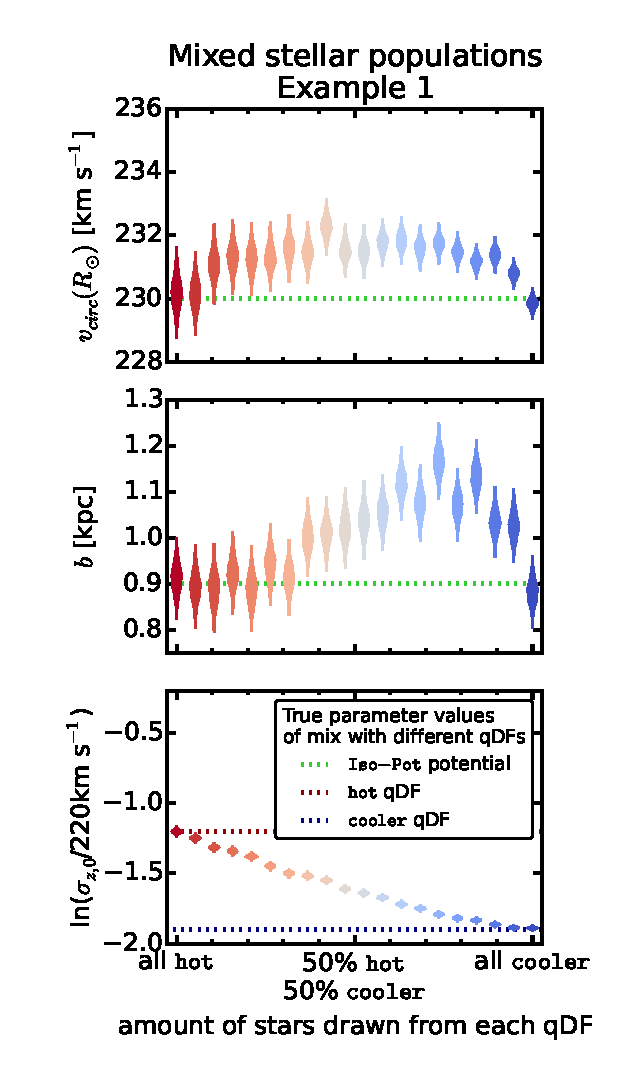
\includegraphics[scale=0.45]{figs/isoSphFlexMixCont_violins_2.eps}
\caption{The dependence of the parameter recovery on degree of pollution and temperature of the stellar population. We mix (i.e., ``pollute'') varying amounts of stars from a \texttt{hot} stellar population with stars from a very different \texttt{cooler} population (see Table \ref{tbl:referenceMAPs}), as indicated on the $x$-axis. (All model parameters used to create the mock data are given as Test \ref{test:isoSphFlexMix}, \emph{Example 1}, in Table \ref{tbl:tests}.) The composite polluted mock data set follows a true DF that has a slightly different shape than the qDF. We then analyse it using \RM{} and fit a \emph{single} qDF only. The violins represent the marginalized \pdf{}s for the best fit model parameters.  Some mock data sets are shown in Figure \ref{fig:isoSphFlexMix_mockdata_residuals}, first row, in the same colors as the violins here.  We find that a hot population is much less affected by pollution with stars from a cooler population than vice versa.}
\label{fig:isoSphFlexMixCont}
\end{figure}



%FIGURE: isoSphFlexMixDiff

\begin{figure}[!htbp]
\centering
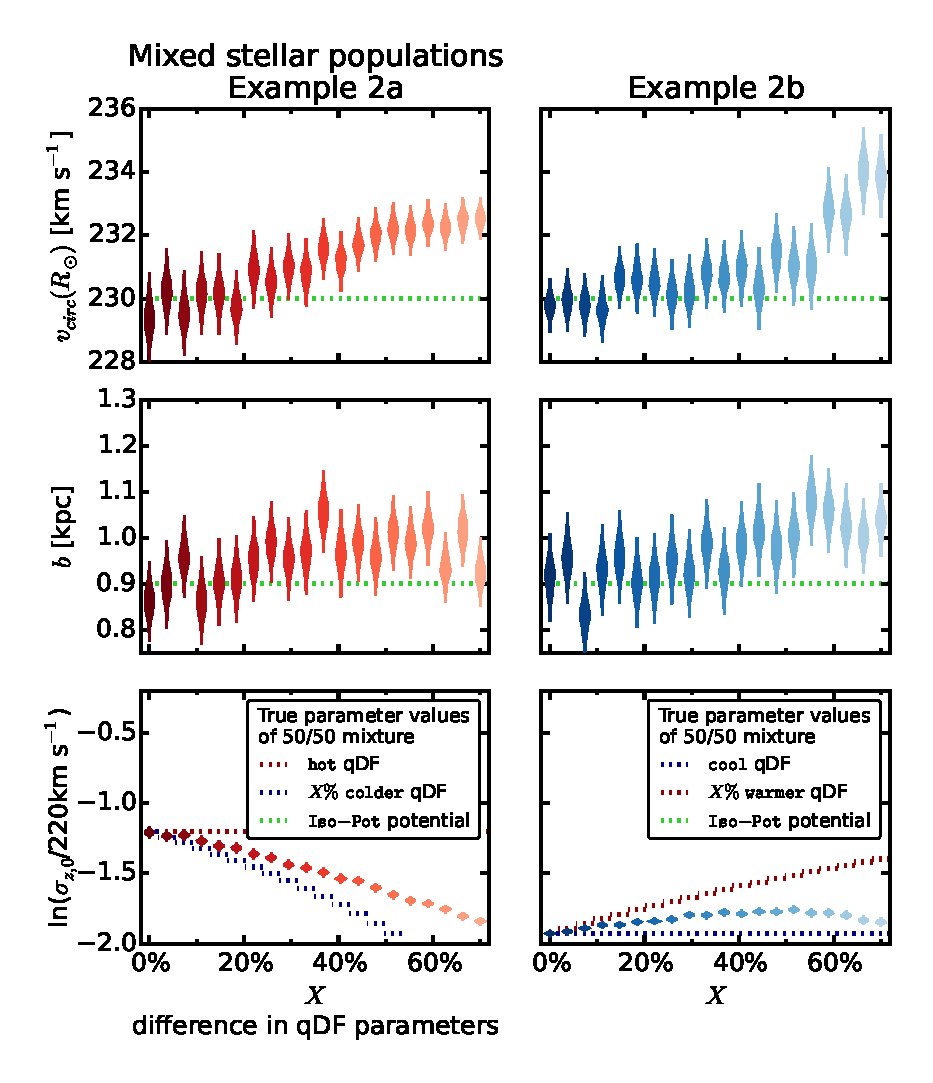
\includegraphics[scale=0.45]{figs/isoSphFlexMixDiff_violins_2.eps}
\caption{The dependence of the parameter recovery on the difference in qDF parameters of a 50/50 mixture of two stellar populations and their temperature. The two qDFs from which the stars in each mock data set were drawn are indicated in the legend, with the qDF parameters $\sigma_{R,0}, \sigma_{z,0}$ and $h_R$ differing by $X\%$ (see also Table \ref{tbl:referenceMAPs}), as indicated on the $x$-axis. (The model parameters used for the mock data creation are given as Test \ref{test:isoSphFlexMix}, \emph{Example 2a \& b}, in Table \ref{tbl:tests}.) Each composite mock data set is fitted with a \emph{single} qDF and the marginalized \pdf{}s are shown as violins. Some mock data sets of Example 2a are shown in Figure \ref{fig:isoSphFlexMix_mockdata_residuals}, last row (color-coded analogous to the violins here). By mixing populations with varying difference in their qDF parameters, we model the effect of finite bin size or abundance errors when sorting stars into different \MAPs{} in the $[\alpha/\mathrm{Fe}]$-vs.-$[\mathrm{Fe}/\mathrm{H}]$ plane and assuming they follow single qDFs (cf. BR13). We find that the bin sizes should be chosen such that the difference in qDF parameters between neighbouring \MAPs{} is less than 20\%.} 
\label{fig:isoSphFlexMixDiff}
\end{figure}

%====================================================================

%============================================================

%FIGURE: isoSphFlexMix_mockdata_residuals

\begin{figure}[!htbp]
\centering
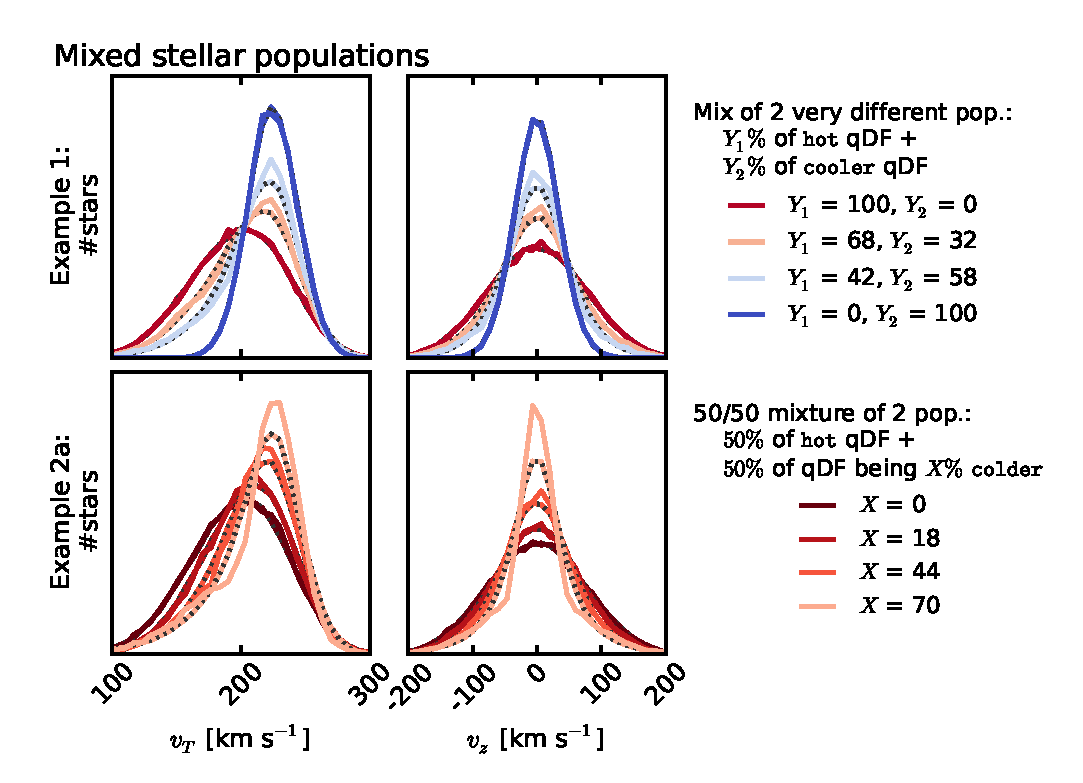
\includegraphics[width=\columnwidth]{figs/isoSphFlexMix_mockdata_residuals_2.eps}
\caption{Distribution of mock data $v_T$ and $v_z$ created by mixing stars drawn from two different qDFs (solid lines), and the distribution predicted by the best fit of a single qDF and potential to the data (dotted lines). (The model parameters used to create the mock data are given in Table \ref{tbl:tests} as Test \ref{test:isoSphFlexMix}, \emph{Example 1 \& 2a}, with the qDF parameters refereed to in the legend given in Table \ref{tbl:referenceMAPs}.) The corresponding single qDF best-fit curves were derived from the best fit parameters found in Figures \ref{fig:isoSphFlexMixCont} and \ref{fig:isoSphFlexMixDiff}. (The data sets are color-coded in the same way as the corresponding analyses in Figures  \ref{fig:isoSphFlexMixCont} and \ref{fig:isoSphFlexMixDiff}.) We use the mixtures of two qDFs to demonstrate how \RM{} behaves for data sets following DFs with shapes slightly differing from a single qDF. For large deviations it might already become visible from directly comparing the mock data and best fit distribution, that a single qDF is a bad assumption for the stars' true DF.}
\label{fig:isoSphFlexMix_mockdata_residuals}
\end{figure}

%============================================================


We consider the impact of the DF deviations on the recovery of the potential and of the qDF parameters separately. 

We find from \emph{Example 1} that the potential parameters can be more robustly recovered, if a mock data population is polluted by a modest fraction ($\lesssim 30\%$) of stars drawn from a much cooler qDF, as opposed to the same pollution of stars from a hotter qDF. When considering the case of a 50/50 mix of contributions from different qDFs in \emph{Example 2}, there is a systematic, but mostly small, bias in recovering the potential parameters, monotonically increasing with the qDF parameter difference. In particular for fractional differences in the qDF parameters of $\lesssim 20\%$ the systematics are insignificant even for sample sizes of $N_{*} = 20,000$, as used in the mock data.

Overall, the circular velocity at the sun is very reliably recovered to within $2\%$ in all these tests. But the best fit $v_\text{circ}(R_\odot)$ is not always unbiased at the implied precision.

The recovery of the effective qDF parameters, in light of non-qDF mock data, is quite intuitive (in Figures \ref{fig:isoSphFlexMixCont} and \ref{fig:isoSphFlexMixDiff} we therefore show only $h_R$): the effective qDF temperature lies between the two temperatures from which the mixed DF of the mock data was drawn; in all cases the scale lengths of the velocity dispersion fall-off, $h_{\sigma,R}$ and $h_{\sigma,z}$, are shorter than the true scale lengths, because the stars drawn form the hotter qDF dominate at small radii, while stars from the cooler qDF (with its longer tracer scale length) dominate at large radii; the recovered tracer scale lengths, $h_R$, vary smoothly between the input values of the two qDFs that entered the mix of mock data, with again the impact of contamination by a hotter qDF (with its shorter scale length in this case) being more important. 

We note, that in the cases where the systematic bias in the potential parameter recovery becomes several sigma large, a direct comparison of the true mock data set and best fit distribution (see Figure \ref{fig:isoSphFlexMix_mockdata_residuals}) can sometimes already reveal that the assumed DF is not a good model for the data.

Overall, we find that the potential inference is quite robust to modest deviations of the data from the assumed DF. 


